\documentclass{beamer}

\usetheme{Torino}
\AtBeginSection[] 
{ 
  \begin{frame}<beamer> 
    \frametitle{Agenda} 
    \tableofcontents[currentsection] 
  \end{frame} 
}  % for recurrent Agenda slide
\numberwithin{equation}{section} % Number equations with sections



\usepackage{amsmath}
\usepackage{amsfonts}
\usepackage[latin1]{inputenc}
\usepackage{amsmath}
\usepackage{amsfonts}
\usepackage{amssymb}
\usepackage{makeidx}
\usepackage{tabularx}
\usepackage{url}
\usepackage[toc,acronym,description]{glossaries}
\usepackage{cite}
\usepackage{hyperref}
\usepackage[noend,boxed,fillcomment]{algorithm2e}
\usepackage{multicol}
\usepackage{fancyvrb}
\usepackage{color}
\usepackage{subfigure}
% use \usepackage[pdfborder=0in]{hyperref} instead to disable red box links
%\usepackage[T1]{fontenc}
\newcommand{\BibTeX}{{\sc Bib}\TeX}
\newcommand{\rischintegrate}{\texttt{risch\_integrate()}}
\hyphenation{Sym-Py an-ti-der-iv-a-tive an-ti-der-iv-a-tives
an-ti-diff-er-en-tia-tion Goo-gle arc-trig-o-no-met-ric
non-el-e-men-tary}

\title{Report on the Risch Algorithm for Symbolic
Integration and Implementation in the SymPy Computer Algebra System}
\author{Aaron Meurer}
\date{December 9, 2010}

\begin{document}

\begin{frame}
    \titlepage
\end{frame}

\begin{frame} 
    \frametitle{Agenda} 
    \tableofcontents 
\end{frame} 

\section{Background}
\subsection{Definitions}

\begin{frame}
    \frametitle{Definitions}
    \begin{itemize}
        \item {\bf Integration} 
        \begin{itemize}
            \item One of two fundamental operations in calculus (the other
            being differentiation).
            \item Informally, $\int_a^b{f(x)\,dx}$ represents the area under
            the curve defined by the function $f(x)$ from the points $x=a$
            to $x=b$.
            \item The Fundamental Theorem of Calculus states that
            integration and antidifferentiation, the inverse operation of
            differentiation, are essentially the same thing.
            \end{itemize}
    \pause
        \item {\bf Algebraic}
        \begin{itemize}
            \item A function is algebraic if it is the root of a polynomial
            with coefficients that are rational functions with rational
            number coefficients.  
            \item For example, the function $\sqrt{x + 1}$ is algebraic
            because it is the root of the polynomial $y^2 = x + 1$. 
        \end{itemize}
    \end{itemize}
\end{frame}

\begin{frame}
    \frametitle{Definitions}
    \begin{itemize}
        \item {\bf Transcendental}
        \begin{itemize}
            \item A function is transcendental if it is not algebraic.  
            \item A function is \textit{purely transcendental} if it does
            not contain any algebraic components.  
            \item $e^x$, $\ln{x}$, $\sin{x}$, $\cos{x}$, and $\tan{x}$ are
            all transcendental.  
            \item Roughly speaking, a function is transcendental if it
            contains one of these, and it is purely transcendental if it
            does not contain any radicals.
            \begin{itemize}
                \item $e^{x + 1}$ is purely transcendental
                \item $\sqrt[3]{\ln{x}}$ is transcendental but not
                purely transcendental
                \item $\sqrt{x}$ is neither transcendental nor purely
                transcendental (it is algebraic)
            \end{itemize}
        \end{itemize}
    \end{itemize}
\end{frame}

\begin{frame}
    \frametitle{Definitions}
    \begin{itemize}
        \item {\bf Elementary}
        \begin{itemize}
            \item Roughly speaking, a function is elementary if it can
            be represented as a combination of exponentials, logarithms,
            powers, and trigonometric functions by addition,
            subtraction, multiplication, division, and composition. 
            \item For example, $\frac{\sin{(x^2 +
            1)}}{\sqrt[3]{\ln{x}}}$ is elementary, but
            $\frac{2}{\sqrt{\pi}}\int{e^{-x^2}\,dx}$, the error
            function, is not.
        \end{itemize}
    \end{itemize}
\end{frame}

\section{The Risch Algorithm}

\subsection{Liouville's Theorem}

\begin{frame}
    \frametitle{Liouville's Theorem}
    \begin{itemize}
        \item If a function $f$ has an elementary integral, then the
        integral can always be written in the form
        \begin{equation}
            \label{liouville's theorem}
            \int{f} = v + \sum_{n=1}^n{c_i\ln{u_i}}
        \end{equation}
        where $v$ and the $u_i$ are ``parts'' of $f$, and the $c_i$ are
        constants.
        \pause
        \item In other words, if we can show that $\int{f}$ does not
        have this form, then we have shown that it is not elementary.
    \end{itemize}
\end{frame}

\subsection{The Transcendental Algorithm}

\begin{frame}
    something
\end{frame}

\section{Implementation in SymPy}

\begin{frame}
    \begin{figure}
    \subfigure{
\includegraphics[width=.32\textwidth]{python-logo-master-v3-TM.png}}
    \subfigure{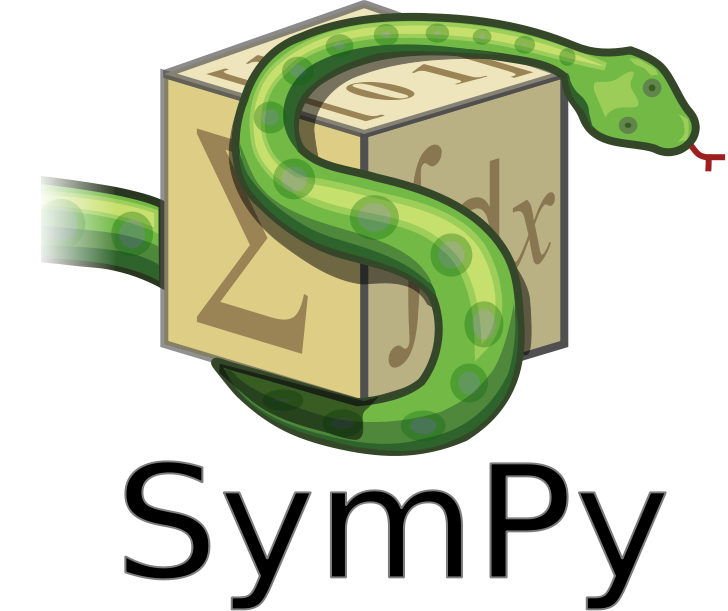
\includegraphics[width=.32\textwidth]{sympy.png}}
   \subfigure{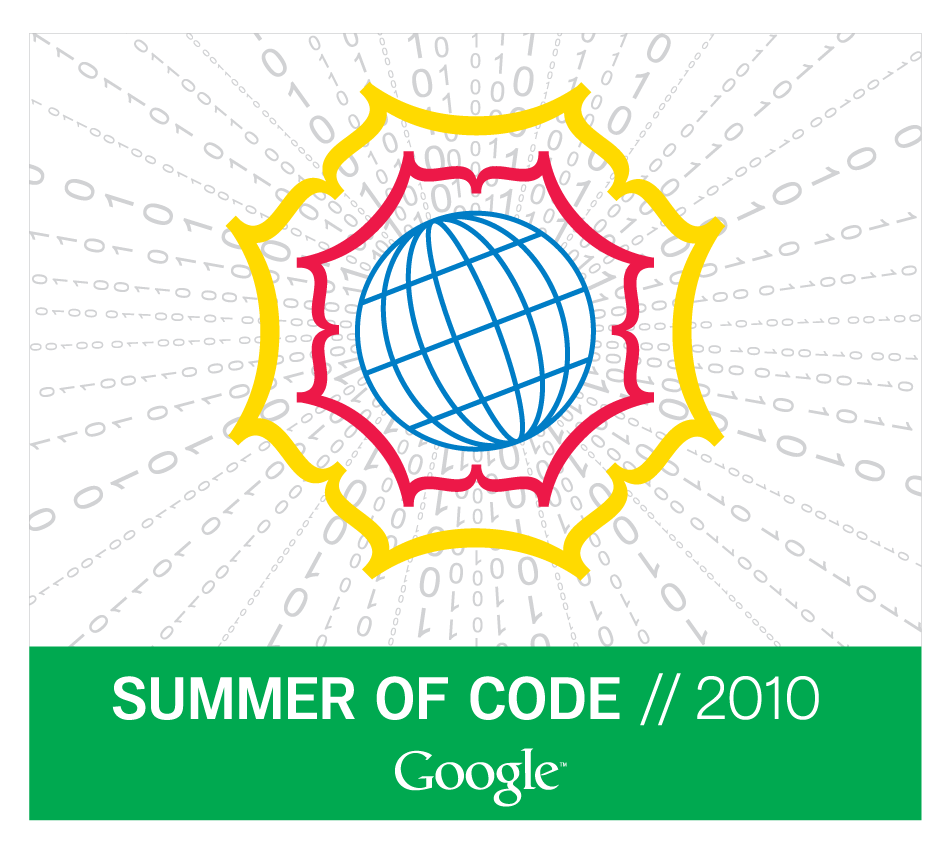
\includegraphics[width=.32\textwidth]{GSoC_2010_logo/2010_NoURL_950x846px.png}}
   \end{figure}

    Over the summer of 2010, I worked for the Python Software
    Organization with the SymPy project under the Google Summer of Code
    program.
\end{frame}

\section{Future}

\begin{frame}

\end{frame}


\section{Questions}

\begin{frame}
    \frametitle{Questions?}
    \huge{Questions?}
\end{frame}

\end{document}
